\chapter{Propuesta de soluci�n}\label{c:chapter2}

\section*{Introducci�n del cap�tulo}
 El presente cap�tulo aborda las particularidades del sistema de gesti�n a desarrollar. Para registrar las principales caracter�sticas se hace uso de los \ac{rf} y \ac{rnf}. Estos describen las funcionalidades y atributos de calidad que debe poseer el software. En el cap�tulo \ref{c:chapter1}, se seleccion� la metodolog�a \ac{xp} como gu�a para el desarrollo del software; por lo tanto, se utilizan las \ac{hu} como herramienta para una descripci�n detallada de los \ac{rf} y la confecci�n del plan de iteraciones. Mediante el uso de este �ltimo, se proceder� a la estimaci�n del tiempo requerido para la culminaci�n del desarrollo del sistema y, con el uso de patrones de dise�o, se facilitar� la posterior descripci�n de las tarjetas \ac{crc}.
 
\section{Requisitos}\label{s:req}

\subsection{Requisitos funcionales}
En ingenier�a de software, los \ac{rf} definen un sistema o sus componentes; describen la funci�n que un software debe realizar, ya sean c�lculos, manipulaci�n de datos, procesos de negocios, entre otros.
Ayudan adem�s a capturar los comportamientos planificados para un sistema, este comportamiento puede ser expresado como una funci�n, servicio o tarea que un software debe realizar~\citep{requisitos}. A continuaci�n, se exponen los diferentes \ac{rf} planteados por el usuario:
\begin{RF}
\item Autenticar Usuario
\item Asignar rol a usuario
\\
\item Listar denuncias
\item Crear denuncia
\item Modificar denuncia
\item Eliminar denuncia
\item Buscar denuncia
%\item Exportar listado de denuncias
%\item Imprimir denuncia
%\item Imprimir listado de denuncias
\\
\item Listar resoluciones
\item Crear resoluci�n
\item Modificar resoluci�n
\item Eliminar resoluci�n
\item Exportar resoluci�n
\\
\item Listar comisiones
\item Crear comisi�n
\item Modificar comisi�n
\item Eliminar comisi�n
\item Buscar comisi�n
\\
\item Listar declaraciones
\item Crear declaraci�n
\item Modificar declaraci�n
\item Eliminar declaraci�n
\item Buscar declaraci�n
%\item Exportar declaraci�n
\\
\item Listar casos disciplinarios
\item Crear caso disciplinario
\item Modificar caso disciplinario
\item Buscar caso disciplinario
\\
\item Exportar Resoluci�n de caso
\item Exportar Expediente
\\
\item Listar roles
\item Crear rol
\item Modificar rol
\item Eliminar rol
\item Buscar rol
\end{RF}

\subsection{Requisitos no funcionales}
Los \ac{rnf}, como su nombre sugiere, son aquellos requerimientos que no se refieren directamente a las funciones espec�ficas que proporciona el sistema, sino a las propiedades emergentes de este como la fiabilidad, el tiempo de respuesta y la capacidad de almacenamiento. De forma alternativa definen las restricciones del sistema \citep{sommerville2011software}.\\
Los requisitos no funcionales de la aplicaci�n a desarrollar son:
\\
\noindent Usabilidad:
\begin{RNF}
\item El sistema debe ser una aplicaci�n web
\item La interfaz del sistema debe ser intuitiva y f�cil de usar
\end{RNF}
Hardware y software:
\begin{RNF}[resume]
\item El sistema operativo del servidor debe tener instalado la m�quina virtual de Java 
\item El ordenador donde se ejecute el servidor debe poseer como m�nimo 4GB de \ac{ram} y 10GB de almacenamiento.
\item El cliente del sistema se podr� ejecutar en los principales navegadores web: Google Chrome y navegadores basados en \gls{chromium}, Mozilla Firefox y Safari.
\end{RNF}
Seguridad:
\begin{RNF}[resume]
\item Solo se podr� acceder al sistema despu�s de estar autenticado con usuario y contrase�a v�lidos
\item Solo se podr�n usar las funcionalidades del sistema en dependencia de si el usuario autenticado posee los permisos requeridos para la misma
\end{RNF}
Dise�o e implementaci�n:
\begin{RNF}[resume]
\item Usar JavaScript como lenguaje de programaci�n del lado del cliente.
%\item Usar VueJS como marco de trabajo de desarrollo del lado del cliente.
\item Usar Java como lenguaje de programaci�n del lado del servidor.
\item Usar Spring Boot como \gls{framework} de desarrollo del lado del servidor.

\item Usar la metodolog�a de desarrollo de software \ac{xp}
\end{RNF}

\section{Historias de usuario}
\label{s:hu}
Las HU ser�n representadas mediante tablas divididas por las siguientes secciones:
\begin{description}

	\item [N�mero] Identificador entero incremental en el tiempo;
	\item [Nombre de historia de usuario] Identificador alfanum�rico para su uso
	      entre los desarrolladores y el cliente;
	\item[Usuario] Nombre y apellidos de la persona involucrada en el desarrollo de la \ac{hu};
	\item[Iteraci�n asignada] Identificador entero perteneciente a la iteraci�n en la cual se planea implementar la funcionalidad descrita en la \ac{hu};
	\item[Prioridad en negocio] Las historias de usuarios que describen funcionalidades imprescindibles en el desarrollo del sistema tienen prioridad alta; aquellas que debe tener el sistema, pero que no son necesarias para su funcionamiento, prioridad media; y auxiliares y que son independientes del sistema, prioridad baja.
	\item[Riesgo en desarrollo] Las historias de usuarios que, en caso de tener alg�n error de implementaci�n, puedan afectar la disponibilidad del sistema, tienen un riesgo de desarrollo alto; las \ac{hu} que puedan presentar errores y retrasan la entrega de la versi�n tienen riesgo de desarrollo medio; y las que puedan presentar errores, pero estos son tratados con facilidad y no afectan en desarrollo del proyecto, tienen riesgo de desarrollo bajo.

	\item[Puntos estimados] Tiempo estimado que tardar� el desarrollo de la \ac{hu};
	\item[Descripci�n] Breve descripci�n de \ac{hu};
	\item[Observaciones] Se�alamiento o advertencia del sistema;
	\item[Prototipo de interfaz] Prototipo de interfaz si aplica.
\end{description} \citep{Joskowicz2008}


Los t�tulos de las \ac{hu} generadas son:
\begin{enumerate}[label=HU \arabic*:]

	\item Autenticar Usuario (Prioridad Alta)

	\item Asignar rol a usuario (Prioridad Baja)

	\item Listar denuncias (Prioridad Alta)

	\item Crear una denuncia (Prioridad Alta)

	\item Modificar una denuncia (Prioridad Alta)

	\item Eliminar denuncias (Prioridad Alta)

	\item Buscar denuncias (Prioridad Baja)

	\item Archivar denuncias (Prioridad Alta)

	\item Listar resoluciones decanales (Prioridad Alta)

	\item Crear una resoluci�n decanal (Prioridad Alta)

	\item Modificar una resoluci�n decanal (Prioridad Alta)

	\item Eliminar resoluciones decanales (Prioridad Alta)

	\item Listar comisiones (Prioridad Alta)

	\item Crear comisiones (Prioridad Alta)

	\item Modificar una comisi�n (Prioridad Alta)

	\item Eliminar comisiones (Prioridad Alta)

	\item Buscar comisiones (Prioridad Baja)

	\item Listar declaraciones (Prioridad Alta)

	\item Crear declaraci�n (Prioridad Alta)

	\item Modificar declaraci�n (Prioridad Alta)

	\item Eliminar declaraciones (Prioridad Alta)

	\item Buscar declaraci�n (Prioridad Baja)

	\item Crear caso disciplinario (Prioridad Alta)

	\item Listar casos disciplinarios (Prioridad Alta)

	\item Modificar caso disciplinario (Prioridad Alta)

	\item Buscar caso disciplinario (Prioridad Baja)

	\item Cerrar caso disciplinario (Prioridad Media)

	\item Listar roles (Prioridad Baja)

	\item Crear roles (Prioridad Baja)

	\item Modificar roles (Prioridad Baja)

	\item Eliminar roles (Prioridad Baja)

	\item Buscar roles (Prioridad Baja)

	\item Exportar resoluciones decanales (Prioridad Baja)

	\item Exportar denuncias (Prioridad Baja)

	\item Exportar declaraciones (Prioridad Baja)

	\item Exportar conclusiones de casos (Prioridad Baja)

	\item Exportar resoluciones de casos (Prioridad Baja)

\end{enumerate}
A continuaci�n se presentan las \ac{hu} con mayor prioridad dentro del negocio, determinadas por el cliente e conjunto con el equipo de desarrollo. El resto se podr�n encontrar en la secci�n de ap�ndices \ref{app:hu}: Historias de Usuario.


\begin{userstory}
	\storyname{ Crear una denuncia }
	\storyuser{ Usuario }
	\storyiter{ 1 }
	\storypriority{ Alta }
	\storyrisk{ Medio }
	\storypoints{ 0.4 }
	\storyprogrammer{ \authorA }
	\storydescription{ Como Usuario quiero crear una denuncia para notificar r�pidamente al decano de una indisciplina cometida por uno o varios estudiantes }
	\storyobservation{ }
	\storyinterface{ 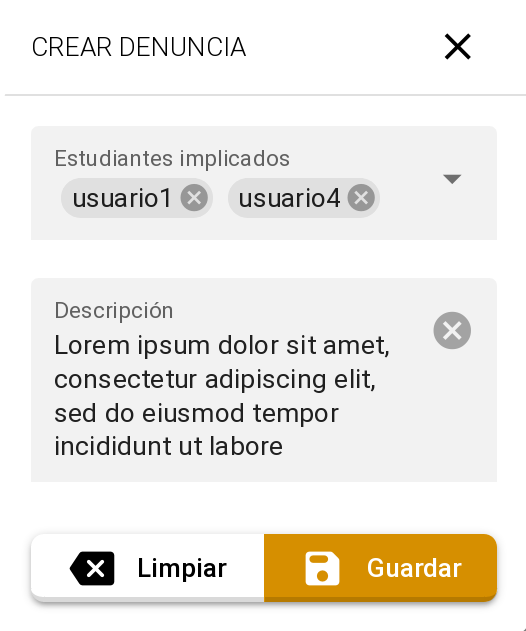
\includegraphics[width=0.5\textwidth]{images/prototypes/cdis-create-denuncia-capture.png} }
\end{userstory}

% Para crear un caso disciplinario basta con asignar una comisi�n a una denuncia pendiente:
% \begin{userstory}
% 	\storyname{ Crear caso disciplinario }
% 	\storyuser{ Decano }
% 	\storyiter{ 1 }
% 	\storypriority{ Alta }
% 	\storyrisk{ Medio }
% 	\storypoints{ 0.4 }
% 	\storyprogrammer{ \authorA }
% 	\storydescription{ Como Decano quiero crear caso disciplinario. }
% 	\storyobservation{ }
% 	\storyinterface{ 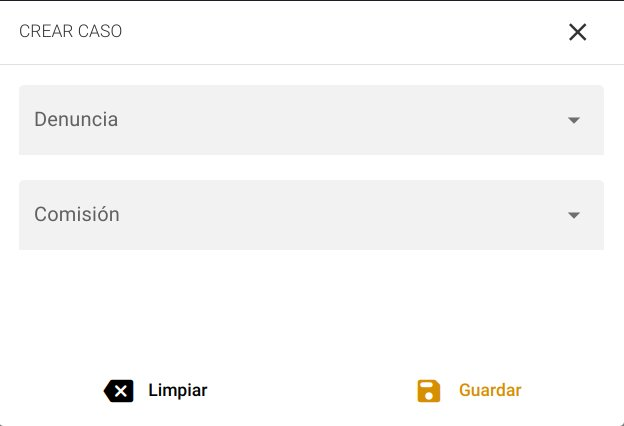
\includegraphics[width=0.5\textwidth]{images/prototypes/cdis-create-caso.png} }
% \end{userstory}
\section{Estimaci�n de esfuerzo por historia de usuario}
\begin {effortestimation}
\addentry[1]{ Listar denuncias }{0.2}
\addentry[1]{ Crear denuncia }{0.4}
\addentry[1]{ Modificar denuncia }{0.4}
\addentry[1]{ Eliminar denuncia }{0.4}

\addentry[1]{ Listar comisiones}{0.2}
\addentry[1]{ Crear comisi�n }{0.4}
\addentry[1]{ Modificar comisi�n }{0.4}
\addentry[1]{ Eliminar comisi�n }{0.4}

\addentry[1]{ Listar resoluciones }{0.2}
\addentry[1]{ Crear resoluci�n }{0.4}
\addentry[1]{ Modificar resoluci�n }{0.4}
\addentry[1]{ Eliminar resoluci�n }{0.4}

\addentry[2]{ Modificar roles de usuario }{0.2}
\addentry[2]{Listar rol}{0.2}
\addentry[2]{Crear rol}{0.4}
\addentry[2]{Modificar rol}{0.4}
\addentry[2]{Eliminar rol}{0.2}

\addentry[3]{ Exportar resoluci�n }{0.6}
\addentry[3]{ Exportar expediente }{0.6}
\end{effortestimation}
%\geniterationplan

\pagebreak
\section{Tarjetas CRC}\label{crc}


\begin{crccard}
   \crcclass{DenunciaController}
   \crcresp{
      \begin{itemize}
         \item crear: Crear una denuncia, la misma se archiva junto con el listado de acusados
         \item listar: Mostrar la denuncia requerida
         \item modificar: Modificar denuncia
         \item borrar: Eliminar denuncia
      \end{itemize}
   }
   \crccolab{
      UsuarioService\\
      DenunciaService\\
      Convertidor\\
      SesionDetails\\
      ValidatorDenuncia\\
      DenunciaUsuarioService\\
      ExpedienteService\\
      CasoUsuarioService\\
      JsonBorrarDenuncia\\
      JsonCrearDenuncia\\
      JsonModificarDenuncia\\
      E\_Denuncia\\
      Mensaje\\
      CasoUsuario\\
      Denuncia\\
      DenunciaUsuario\\
      Usuario\\
   }
\end{crccard}

\begin{crccard}
   \crcclass{ExpedienteController}
   \crcresp{
      \begin{itemize}
         \item listar: Mostrar todos los expedientes de cada estudiante denunciado
         \item modificar: Editar la informaci�n contenida en cada expediente
      \end{itemize}
   }
   \crccolab{
      JsonModificarExpediente\\
      E\_Expediente\\
      ValidatorExpediente\\
      Convertidor\\
      Mensaje\\
      Expediente\\
      ExpedientePK\\
      ExpedienteService\\
   }
\end{crccard}

\begin{crccard}
   \crcclass{ResolucionController}
   \crcresp{
      \begin{itemize}
         \item crear: Crear la resoluci�n con todas las comisiones disciplinarias que conlleva
         \item mostrar: Mostrar todas las resoluciones
         \item borrar: Eliminar una resoluci�n
         \item modificar: Editar una resoluci�n
      \end{itemize}
   }
   \crccolab{
      JsonBorrarResolucion\\
      E\_ExpedienteJsonCrearResolucion\\
      ComisionReducida\\
      JsonModificarResolucion\\
      E\_Resolucion\\
      ValidatorResolucion\\
      Convertidor\\
      Mensaje\\
      Comision\\
      ComisionUsuario\\
      ComisionUsuarioPK\\
      Resolucion\\
      ComisionService\\
      ComisionUsuarioService\\
      ResolucionService\\
      RolService\\
      UsuarioService\\
   }
\end{crccard}
